%\section{Une section}

% remarque : pour qu'un mot se retrouve dans le lexique : \MotDefinition{asymptote horizontale}{} 

\begin{aconnaitre}
Une \MotDefinition{translation}{} consiste à faire glisser une figure selon un \MotDefinition{vecteur}{} donné.\\[0.5em]
\begin{minipage}[c]{0.62\linewidth}
Un \textbf{vecteur} est représenté par une flèche et est défini par :
\begin{itemize}
 \item une direction (c'est la direction de la droite)
 \item un sens (c'est le sens de la flèche)
 \item une longueur (c'est la longueur du segment)
 \end{itemize}
 \end{minipage} \hfill%
 \begin{minipage}[c]{0.34\linewidth}
 \begin{center}
 %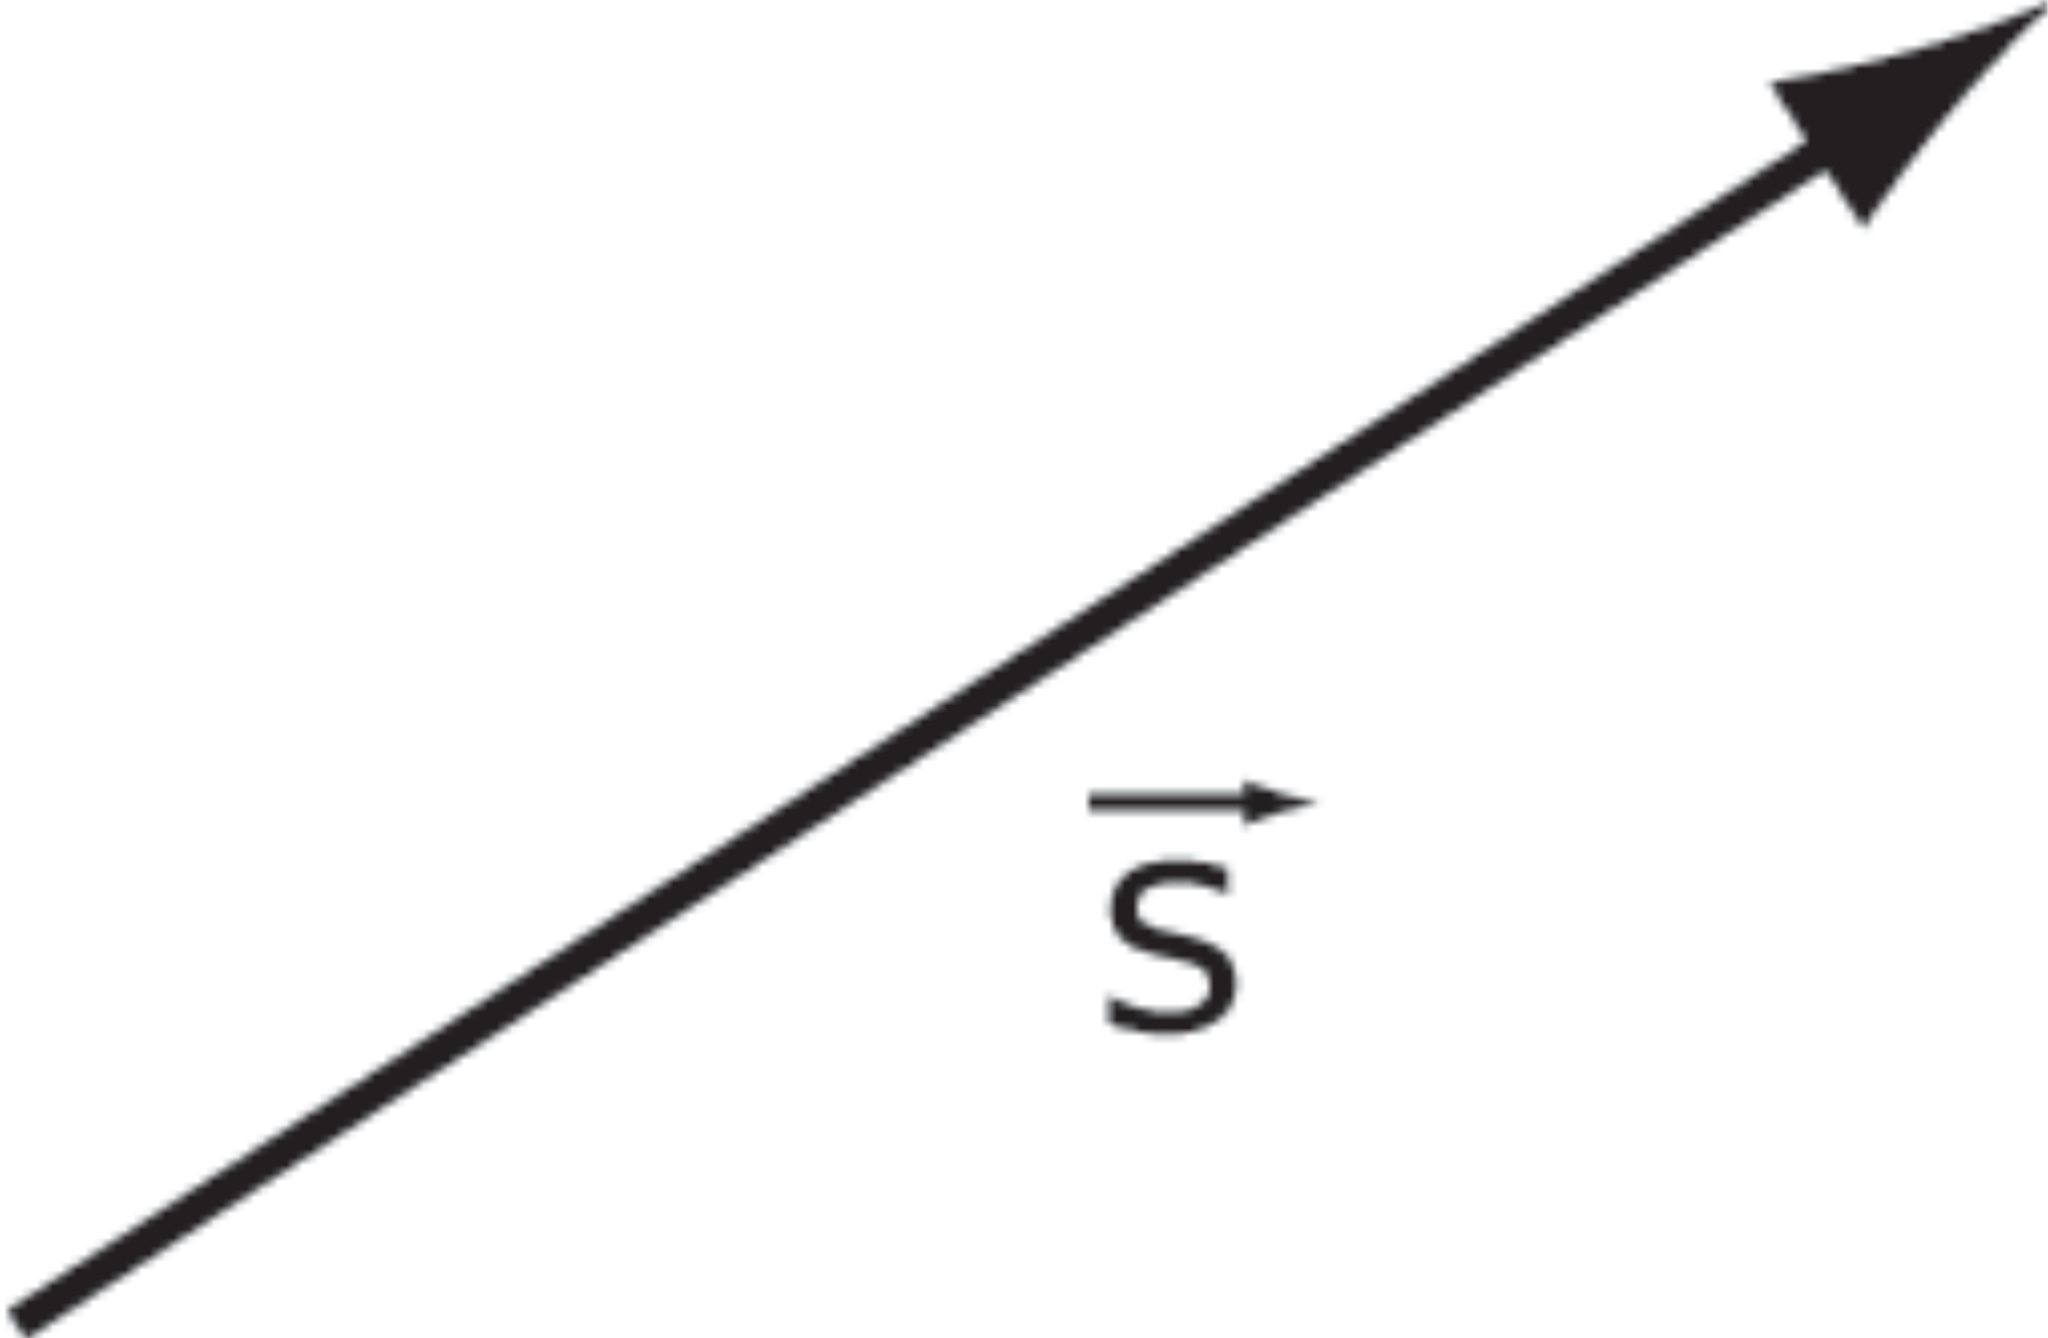
\includegraphics[width=2.3cm]{vecS} 
\scalebox{.8}{
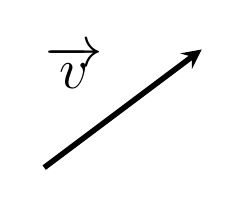
\begin{tikzpicture}
\begin{huge}
\draw [line width = 2pt,>=stealth,->] (0,0) -- (2,1.5) node[midway, above left] {$\overrightarrow{v}$};
\end{huge}
\end{tikzpicture}
} 
 \end{center}
 \end{minipage} \\
\end{aconnaitre}

\begin{remarque}
 Un vecteur peut avoir un nom, écrit avec une seule lettre en minuscule, par exemple $\overrightarrow{v}$ ou $\overrightarrow{s}$. Mais si la flèche qui représente le vecteur part d'un point $D$ et arrive au point $F$, alors on peut aussi appeler le vecteur $\overrightarrow{DF}$.
\end{remarque}


\begin{methode*1}[La translation]
\begin{exemple*1}
Construis l'image du triangle $ABC$ par la translation de vecteur $\vec{a}$ : \hfill
\begin{tabularx}{\linewidth}{X|X|X}
\textcolor{H1}{$\circled{1}$} & \textcolor{H1}{$\circled{2}$} & \textcolor{H1}{$\circled{3}$} \\
\scalebox{.4}{
\definecolor{CouleurPoints}{rgb}{0,0,1}
\begin{tikzpicture}[general,every node/.style={scale=2}]
%Les coordonnées du vecteur
\def \AbscVect {1};
\def \OrdVect {2};
%les sommets des 2 triangles 
\begin{huge}
\coordinate (A) at (3,1.6);
\coordinate (B) at (0,0);
\coordinate (C) at (4.5,-0.5);
%\coordinate (A') at (3+\AbscVect,1.6+\OrdVect);
%\coordinate (B') at (0+\AbscVect,0+\OrdVect);
%\coordinate (C') at (4.5+\AbscVect,-0.5+\OrdVect);
\draw[color=CouleurPoints] (A) node[right] {$A$};
\draw[color=CouleurPoints] (B) node[left] {$B$};
\draw[color=CouleurPoints] (C) node[right] {$C$};
%\draw[color=CouleurPoints] (A') node[right] {$A'$};
%\draw[color=CouleurPoints] (B') node[left] {$B'$};
%\draw[color=CouleurPoints] (C') node[right] {$C'$};

% les 3 cotés des triangles :
\draw[line width = 1.5pt] (A) -- (B) -- (C) -- cycle;
%\draw[line width = 0.4pt] (A') -- (B') -- (C') -- cycle;

%le vecteur de base
\draw [line width = 1.7pt,->] (5.4,0) -- ++(1,2) node[midway,below] {$\overrightarrow{a}$};

%les trois vecteurs partant des sommets
%\draw [>=stealth,->,line width = 1pt] (A) -- (A');
%\draw [>=stealth,->,line width = 1pt] (B) -- (B');
%\draw [>=stealth,->,line width = 1pt] (C) -- (C');

%les droites parallèles au vecteur
\draw[line width = 1.2pt] (A)-- ++(-1.3*\AbscVect,-1.3*\OrdVect) -- ++(2.5*\AbscVect,2.5*\OrdVect);
\draw[line width = 1.2pt] (B)-- ++(-0.5*\AbscVect,-0.5*\OrdVect) -- ++(2.5*\AbscVect,2.5*\OrdVect);
\draw[line width = 1.2pt] (C)-- ++(-0.5*\AbscVect,-0.5*\OrdVect) -- ++(2.5*\AbscVect,2.5*\OrdVect);
\end{huge}
\end{tikzpicture}
} 
 & \input{TranslationsRotations/figures/CoursMethode1_fig2.tex} & \input{TranslationsRotations/figures/CoursMethode1_fig3.tex} \\
\end{tabularx} \\
\textcolor{H1}{$\circled{1}$} On trace des droites parallèles au vecteur $\vec{a}$ passant par les sommets de la figure ;
\textcolor{H1}{$\circled{2}$} On reporte sur les droites le vecteur $\vec{a}$ en respectant le sens donné par la flèche ;
\textcolor{H1}{$\circled{3}$} On relie les sommets entre eux.
 \end{exemple*1}
 
 \begin{exemple*1}
$A'$ est l'image de $A$ par une translation. Construis l'image $B'$ de $B$ par cette translation :
\begin{tabularx}{\linewidth}{X|X|X}
\textcolor{H1}{$\circled{1}$} & \textcolor{H1}{$\circled{2}$} &\textcolor{H1}{$\circled{3}$} \\
\scalebox{.4}{
\begin{tikzpicture}[general,every node/.style={scale=2}]
%Les coordonnées du vecteur
\def \AbscVect {4};
\def \OrdVect {-2};
\begin{huge}
\coordinate (A) at (0,0);
\coordinate (B) at (7,2);
\coordinate (A') at (0+\AbscVect,0+\OrdVect);

\draw (A) node[above right] {$A$};
\draw (A) node{$\times$};
\draw (B) node[left] {$B$};
\draw (B) node{$\times$};
\draw (A') node[right] {$A'$};
\draw (A') node{$\times$};

\end{huge}
\end{tikzpicture}
} 
 & \scalebox{.4}{
\begin{tikzpicture}[general,every node/.style={scale=2}]
%Les coordonnées du vecteur
\def \AbscVect {4};
\def \OrdVect {-2};
\begin{huge}
\coordinate (A) at (0,0);
\coordinate (B) at (7,2);
\coordinate (A') at (0+\AbscVect,0+\OrdVect);

\draw (A) node[above right] {$A$};
\draw (A) node{$\times$};
\draw (B) node[left] {$B$};
\draw (B) node{$\times$};
\draw (A') node[right] {$A'$};
\draw (A') node{$\times$};

%le vecteur de base
\draw [line width = 2pt,>=stealth,->] (A) -- (A') node[midway, above right] {$\overrightarrow{AA'}$};

\end{huge}
\end{tikzpicture}
} 
  & \scalebox{.4}{
\begin{tikzpicture}[general,every node/.style={scale=2}]
%Les coordonnées du vecteur
\def \AbscVect {4};
\def \OrdVect {-2};
\begin{huge}
\coordinate (A) at (0,0);
\coordinate (B) at (7,2);
\coordinate (A') at (0+\AbscVect,0+\OrdVect);
\coordinate (B') at (7+\AbscVect,2+\OrdVect);
\draw (A) node[above right] {$A$};
\draw (A) node{$\times$};
\draw (B) node[left] {$B$};
\draw (B) node{$\times$};
\draw (A') node[right] {$A'$};
\draw (A') node{$\times$};
\draw (B') node[below left] {$B'$};
\draw (B') node{$\times$};

%le vecteur de base
\draw [line width = 2pt,>=stealth,->] (A) -- (A') node[midway, above right] {$\overrightarrow{AA'}$};
%\draw [line width = 2pt,>=stealth,->] (B) -- (B') node[midway, above right] {$\overrightarrow{BB'}$};
\end{huge}
\end{tikzpicture}
} 
\\ 
\end{tabularx} \\
\textcolor{H1}{$\circled{1}$} Les trois points sont donnés ;\\
\textcolor{H1}{$\circled{2}$} on trace d'abord le vecteur $\overrightarrow{AA'}$ ;\\
\textcolor{H1}{$\circled{2}$} on construit l'image du point $B$ par la translation de vecteur $\overrightarrow{AA'}$.
\end{exemple*1}

 \exercice
En t'aidant du quadrillage de ton cahier, reproduis la figure puis construis son imageS par la translation de vecteur $\overrightarrow{b}$ :
\begin{center} \includegraphics[width=4.5cm]{quadrillage_vecB} \end{center}
%\correction

 \end{methode*1}
 
%%%%%%%%%%%%%%%%%%%%%%%%%%%%%%%%%%%%%%%%%%%%%%%%%%%%%%%%%%%%%%%%%%%%%%%

\begin{aconnaitre}
Une \MotDefinition{rotation}{} est définie par son \textbf{centre} et son \textbf{angle}.

L'angle de rotation est \textbf{positif} si la rotation s'effectue dans le sens contraire des aiguilles d'une montre et \textbf{négatif} sinon.
\end{aconnaitre}

\begin{remarque}
La rotation de centre $O$ et d'angle $\alpha$ est notée : $R(O ; \alpha)$.
 \end{remarque}

\begin{methode*1}[La rotation]

 \begin{exemple*1}
 Construis l'image du triangle $ABC$ par la rotation $R(O ; - 45^\circ)$ :
 
%\begin{tabularx}{\linewidth}{X|X}
 %\textcolor{H1}{$\circled{1}$} & \textcolor{H1}{$\circled{2}$} \\
%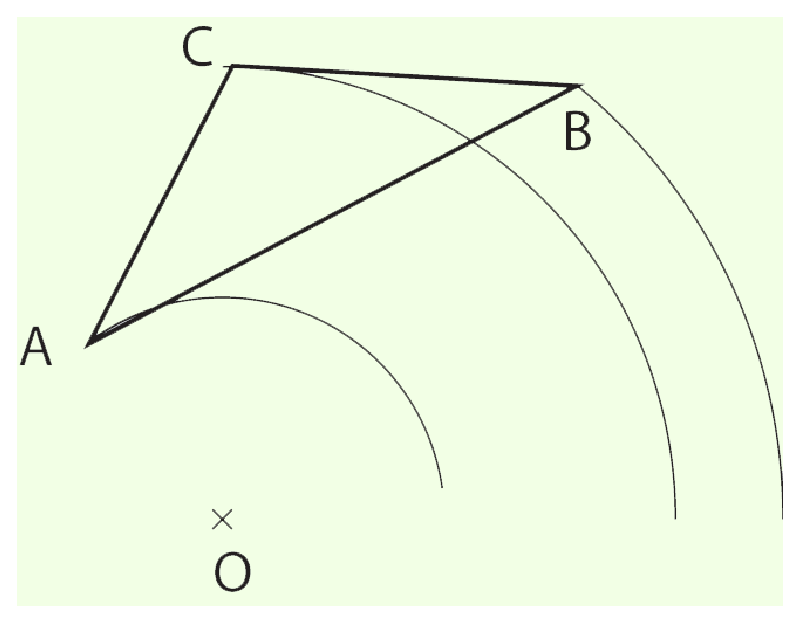
\includegraphics[width=4.7cm]{rotation_triangleABC} &  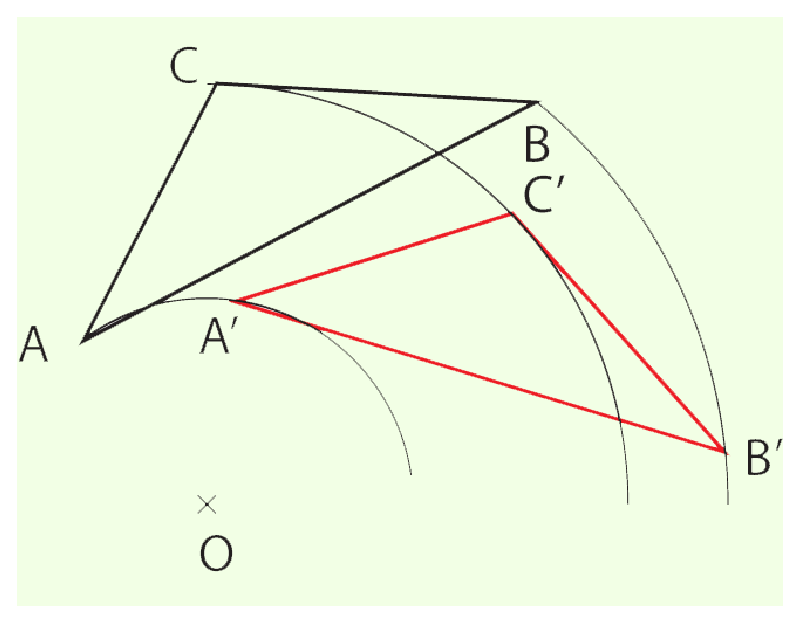
\includegraphics[width=4.7cm]{rotation_triangleABC2} \\ 
%\end{tabularx} \\

\textcolor{H1}{$\circled{1}$} La rotation s'effectue dans le sens des aiguilles d'une montre. On trace des arcs de cercles de centre $O$ passant par les sommets $A$, $B$ et $C$ ;
\textcolor{H1}{$\circled{2}$} On reporte l'angle de rotation sur tous les arcs de cercles ($\widehat{AOA'} = 45^\circ$) et on relie les sommets entre eux.
 \end{exemple*1}
 
\begin{exemple*1}
$A'$ et $B'$ sont l'image de $A$ et $B$ par une rotation. Détermine le centre de la rotation ainsi que l'angle de rotation :

\begin{minipage}[c]{0.44\linewidth}
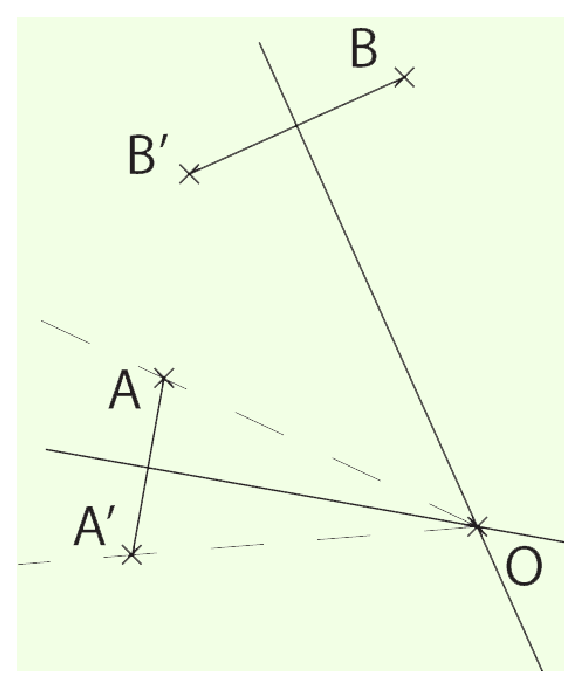
\includegraphics[width=3.7cm]{centre_rotation}
 \end{minipage} \hfill%
 \begin{minipage}[c]{0.52\linewidth}
On trace les médiatrices de $[AA']$ et $[BB']$. L'intersection des médiatrices donne le centre de la rotation $O$. \\[0.5em]
La rotation s'effectue dans le sens inverse des aiguilles d'une montre alors l'angle est positif. L'angle $\widehat{AOA'} = 30^\circ$ donc l'angle de rotation est $+ 30^\circ$
 \end{minipage} \\ 
 \end{exemple*1}

 \exercice
 En t'aidant du quadrillage de ton cahier, reproduis la figure puis construis son image par la rotation $R(O ; -90^\circ)$ : \\[0.5em]
 \begin{center} 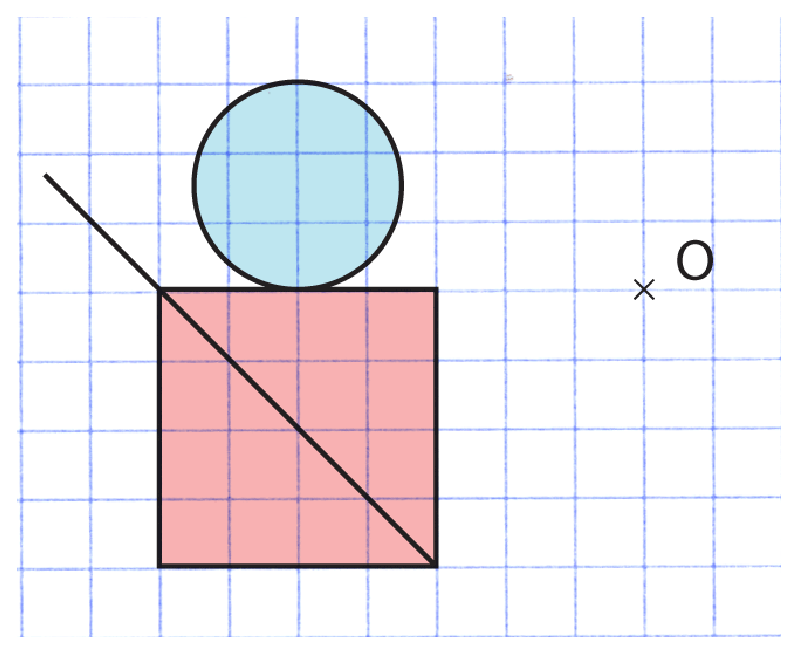
\includegraphics[width=5.2cm]{rotation_O60} \end{center}
%\correction

 \end{methode*1}
 
%%%%%%%%%%%%%%%%%%%%%%%%%%%%%%%%%%%%%%%%%%%%%%%%%%%%%%%%%%%%%%%%%%%%%%%
